\documentclass{article}
%% Выставим минимальные поля, согласно новому ГОСТу:
\usepackage[letterpaper, top = 2cm, bottom = 2cm, left = 2cm, right = 1cm]{geometry}
\usepackage{amsmath}
\usepackage[utf8]{inputenc}
%% Импортируем русский язык:
\usepackage[russian]{babel}
\usepackage{setspace}
\usepackage[pdf]{graphviz}


%% Заголовок, автор и дата:
\title{Теоретические модели вычислений ДЗ №1: Регулярные языки и конечные автоматы}
\author{А-13б-19 Сергей Тимченко}
\date{6 апреля 2022}


\begin{document}

%% Задание №1 
\maketitle
\section{Задание №1. Построить конечный автомат, распознающий язык.}

\begin{enumerate}
    %% 1.1
    \item {$L = \{ w \in \{ a, b, c\}^* \ | \ |w|_c = 1\}$}
    \begin{flushleft}
        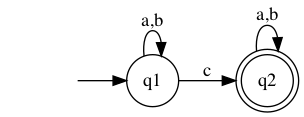
\includegraphics[width=0.5\textwidth]{g1_1.png}
    \end{flushleft}
    %% 1.2
    \item {$L = \{ w \in \{ a, b\}^* \ | \ |w|_a \leq 2, |w|_b \geq 2 \}$} \\ \\
    В данной задаче будем делать через прямое произведение. Для этого построим два отдельных автомата и затем вручную перемножим. \\ \\
    \text{Первый:} \\ \\
    $L_1 = \{ w \in \{ a, b\}^* \ | \ |w|_a \leq 2 \}$
    \begin{flushleft}
        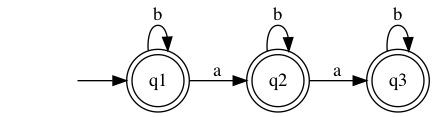
\includegraphics[width=0.7\textwidth]{g1_2_l1.png}
    \end{flushleft}
    \text{Второй:} \\ \\
    $L_2 = \{ w \in \{ a, b\}^* \ | \ |w|_b \geq 2 \}$
    \begin{flushleft}
        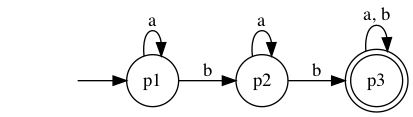
\includegraphics[width=0.7\textwidth]{g1_2_l2.png}
    \end{flushleft}
    $L = L_1 \times L_2$ \\
    $\sum = \{a, b\}$ \\
    $Q = \{q1p1, q1p2, q1p3, q2p1, q2p2, q2p3, q3p1, q3p2, q3p3\}$ \\
    $s = \langle q1, p1 \rangle $ \\
    $T = \{q1p3, q2p3, q3p3\}$ \\ \\
    \begin{tabular}{|c|c|c|}
        \hline
                              & a                         & b     \\ \hline
         $\langle q1,p1 \rangle$    & $\langle q2,p1 \rangle$   & $\langle q1,p2 \rangle$    \\
         $\langle q1,p2 \rangle$    & $\langle q2,p2 \rangle$   & $\langle q1,p3 \rangle$    \\ 
         $\langle q1,p3 \rangle$    & $\langle q2,p3 \rangle$   & $\langle q1,p3 \rangle$    \\
         $\langle q2,p1 \rangle$    & $\langle q3,p1 \rangle$   & $\langle q2,p2 \rangle$    \\
         $\langle q2,p2 \rangle$    & $\langle q3,p2 \rangle$   & $\langle q2,p3 \rangle$    \\ 
         $\langle q2,p3 \rangle$    & $\langle q3,p3 \rangle$   & $\langle q2,p3 \rangle$    \\
         $\langle q3,p1 \rangle$    & -                         & $\langle q3,p2 \rangle$    \\
         $\langle q3,p2 \rangle$    & -                         & $\langle q3,p3 \rangle$    \\ 
         $\langle q3,p3 \rangle$    & -                         & $\langle q3,p3 \rangle$    \\ \hline
    \end{tabular} \\
    
    \text{Построим ДКА:}\\ 
    \begin{flushleft}
        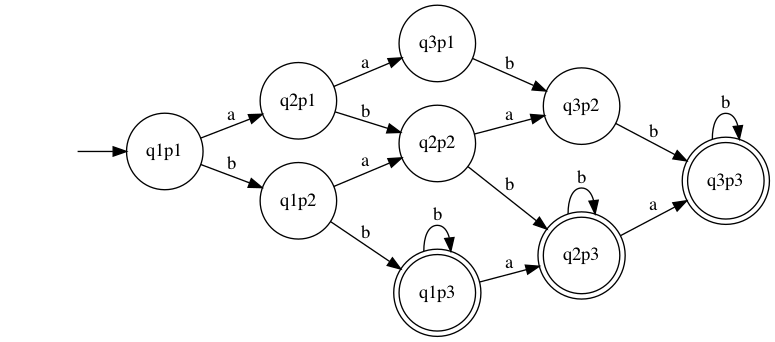
\includegraphics[width=0.9\textwidth]{g1_2.png}
    \end{flushleft}
    %% 1.3 
    \item {$L = \{ w \in \{ a, b\}^* \ | \ |w|_a \neq |w|_b\}$} \\ \\ 
    Нельзя построить детерминированный конечный автомат. В данном случае для построения автомата необходимо запоминать количество символов $a$ и  $b$. Как мы знаем ДКА не способен на это.
    %% 1.4
    \item {$L = \{ w \in \{ a, b\}^* \ | \ { w w = w w w } \}$} \\ \\
    Язык допускает только распознавание пустого слова:
    \begin{flushleft}
        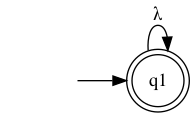
\includegraphics[width=0.3\textwidth]{g1_5.png}
    \end{flushleft}
\end{enumerate}

\section{Задание №2. Построить конечный автомат, используя прямое произведение.}
\begin{enumerate}
    %% 2.1
    \item {$L_1 = \{ w \in \{ a, b\}^* \ | \ |w|_a \geq 2 \wedge |w|_b \geq 2 \}$} \\ \\
    $A = \{ w \in \{ a, b\}^* \ | \ |w|_a \geq 2 \}$
    \begin{flushleft}
        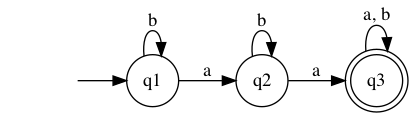
\includegraphics[width=0.7\textwidth]{g2_1_A.png}
    \end{flushleft}
    $B = \{ w \in \{ a, b\}^* \ | \ |w|_b \geq 2 \}$
    \begin{flushleft}
        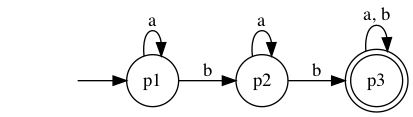
\includegraphics[width=0.7\textwidth]{g2_1_B.png}
    \end{flushleft}
    $L_1 = A \times B$ \\
    $\sum = \{a, b\}$ \\
    $Q = \{q1p1, q1p2, q1p3, q2p1, q2p2, q2p3, q3p1, q3p2, q3p3\}$ \\
    $s = \langle q1, p1 \rangle $ \\
    $T = \{q3p3\}$ \\ \\
    \begin{tabular}{|c|c|c|}
        \hline
                              & a                         & b     \\ \hline
         $\langle q1,p1 \rangle$    & $\langle q2,p1 \rangle$   & $\langle q1,p2 \rangle$    \\
         $\langle q1,p2 \rangle$    & $\langle q2,p2 \rangle$   & $\langle q1,p3 \rangle$    \\ 
         $\langle q1,p3 \rangle$    & $\langle q2,p3 \rangle$   & $\langle q1,p3 \rangle$    \\
         $\langle q2,p1 \rangle$    & $\langle q3,p1 \rangle$   & $\langle q2,p2 \rangle$    \\
         $\langle q2,p2 \rangle$    & $\langle q3,p2 \rangle$   & $\langle q2,p3 \rangle$    \\ 
         $\langle q2,p3 \rangle$    & $\langle q3,p3 \rangle$   & $\langle q2,p3 \rangle$    \\
         $\langle q3,p1 \rangle$    & $\langle q3,p1 \rangle$   & $\langle q3,p2 \rangle$    \\
         $\langle q3,p2 \rangle$    & $\langle q3,p2 \rangle$   & $\langle q3,p3 \rangle$    \\ 
         $\langle q3,p3 \rangle$    & $\langle q3,p3 \rangle$   & $\langle q3,p3 \rangle$    \\ \hline
    \end{tabular} \\
    
    \text{Построим ДКА:}\\ 
    \begin{flushleft}
        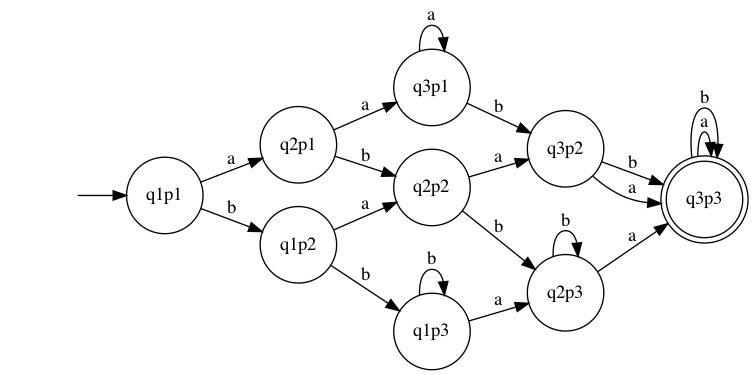
\includegraphics[width=0.7\textwidth]{g2_1.png}
    \end{flushleft}
    %% 2.2
    \item {$L_2 = \{ w \in \{ a, b\}^* \ | \ |w| \geq 3 \wedge |w| \ \text{нечетное} \}$} \\ \\
    $A = \{ w \in \{ a, b\}^* \ | \ |w| \geq 3 \}$
    \begin{flushleft}
        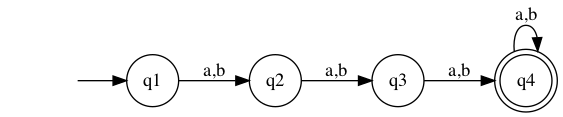
\includegraphics[width=0.8\textwidth]{g2_2_A.png}
    \end{flushleft}
    $B = \{ w \in \{ a, b\}^* \ | \ |w| \ \text{нечетно} \}$
    \begin{flushleft}
        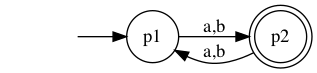
\includegraphics[width=0.7\textwidth]{g2_2_B.png}
    \end{flushleft}
    $L_2 = A \times B$ \\
    $\sum = \{a, b\}$ \\
    $Q = \{q1p1, q1p2, q2p1, q2p2, q3p1, q3p2, q4p1, q4p2\}$ \\
    $s = \langle q1, p1 \rangle $ \\
    $T = \{q4p2\}$ \\ \\
    \begin{tabular}{|c|c|c|}
        \hline
                              & a                         & b     \\ \hline
         $\langle q1,p1 \rangle$    & $\langle q2,p2 \rangle$   & $\langle q2,p2 \rangle$    \\
         $\langle q1,p2 \rangle$    & $\langle q2,p1 \rangle$   & $\langle q2,p1 \rangle$    \\ 
         $\langle q2,p1 \rangle$    & $\langle q3,p2 \rangle$   & $\langle q3,p2 \rangle$    \\
         $\langle q2,p2 \rangle$    & $\langle q3,p1 \rangle$   & $\langle q3,p1 \rangle$    \\ 
         $\langle q3,p1 \rangle$    & $\langle q4,p2 \rangle$   & $\langle q4,p2 \rangle$    \\
         $\langle q3,p2 \rangle$    & $\langle q4,p1 \rangle$   & $\langle q4,p1 \rangle$    \\  
         $\langle q4,p1 \rangle$    & $\langle q4,p2 \rangle$   & $\langle q4,p2 \rangle$    \\
         $\langle q4,p2 \rangle$    & $\langle q4,p1 \rangle$   & $\langle q4,p1 \rangle$    \\ \hline
    \end{tabular} \\
    
    \text{Построим ДКА:}\\ 
    \begin{flushleft}
        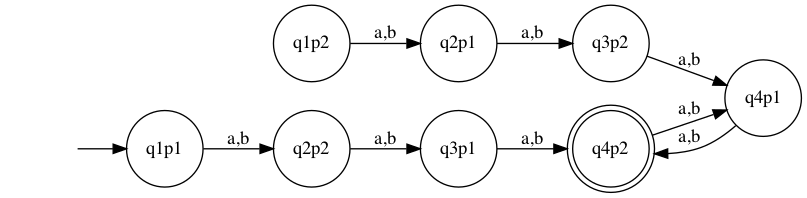
\includegraphics[width=0.7\textwidth]{g2_2.png}
    \end{flushleft}
    %% 3.3
    \item {$L_3 = \{ w \in \{ a, b\}^* \ | \ |w|_a \ \text{четно} \wedge |w|_b \ \text{кратно трем} \}$} \\ \\
    $A = \{ w \in \{ a, b\}^* \ | \ |w|_a \ \text{четно}\}$
    \begin{flushleft}
        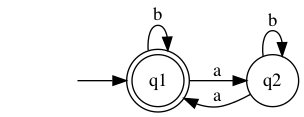
\includegraphics[width=0.8\textwidth]{g2_3_A.png}
    \end{flushleft}
    $B = \{ w \in \{ a, b\}^* \ | \ |w|_b \ \text{кратно трем} \}$
    \begin{flushleft}
        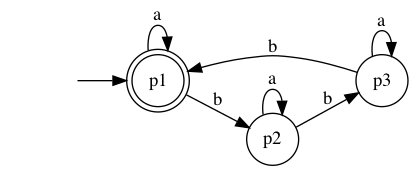
\includegraphics[width=0.8\textwidth]{g2_3_B.png}
    \end{flushleft}
    $L_3 = A \times B$ \\
    $\sum = \{a, b\}$ \\
    $Q = \{q1p1, q1p2, q1p3, q2p1, q2p2, q2p3\}$ \\
    $s = \langle q1, p1 \rangle $ \\
    $T = \{q1p1\}$ \\ \\
    \begin{tabular}{|c|c|c|}
        \hline
                              & a                         & b     \\ \hline
         $\langle q1,p1 \rangle$    & $\langle q2,p1 \rangle$   & $\langle q1,p2 \rangle$    \\
         $\langle q1,p2 \rangle$    & $\langle q2,p2 \rangle$   & $\langle q1,p3 \rangle$    \\ 
         $\langle q1,p3 \rangle$    & $\langle q2,p3 \rangle$   & $\langle q1,p1 \rangle$    \\
         $\langle q2,p1 \rangle$    & $\langle q1,p1 \rangle$   & $\langle q2,p2 \rangle$    \\ 
         $\langle q2,p2 \rangle$    & $\langle q1,p2 \rangle$   & $\langle q2,p3 \rangle$    \\
         $\langle q2,p3 \rangle$    & $\langle q1,p3 \rangle$   & $\langle q2,p1 \rangle$    \\  \hline
    \end{tabular} \\
    
    \text{Построим ДКА:}\\ 
    \begin{flushleft}
        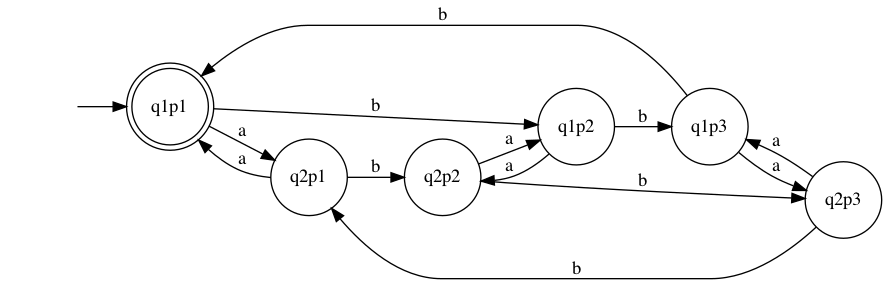
\includegraphics[width=0.8\textwidth]{g2_3.png}
    \end{flushleft}
    %% 2.4
    \item {$L_4 = \overline{L_3} $} \\ \\ 
    Для построения данного автомата воспользуемся уже построенным. Задача сводится к тому, чтобы определить новые конечные вершины. \\ \\
    $T = \{q1p2, q1p3, q2p1, q2p2, q2p3\}$
    \begin{flushleft}
        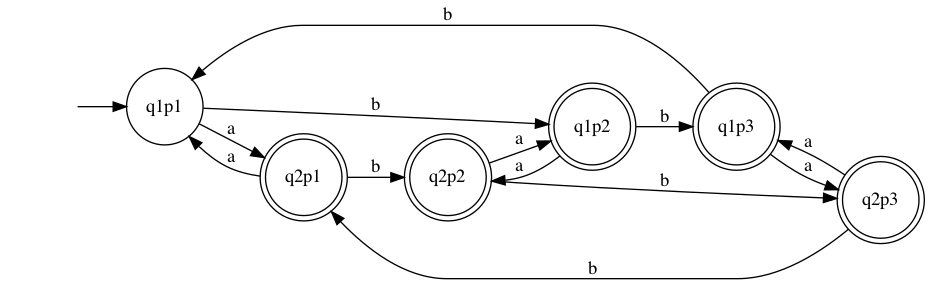
\includegraphics[width=0.8\textwidth]{g2_4.png}
    \end{flushleft}
    \item {$L_5 = L_2 \setminus L_3 $} \\
    Знаем, что
    $$ L_5 = L_2 \setminus L_3 = L_2 \times \overline L_3$$
    Для начала разберемся с $L_2$:
    \begin{flushleft}
        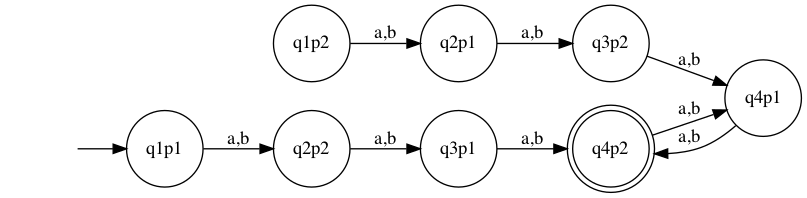
\includegraphics[width=0.8\textwidth]{g2_2.png}
    \end{flushleft}
    Заметим, что $q1p2, q2p1, q3p2$ не будут достигнуты никогда. Поэтому от них можно избавиться в ДКА:
    \begin{flushleft}
        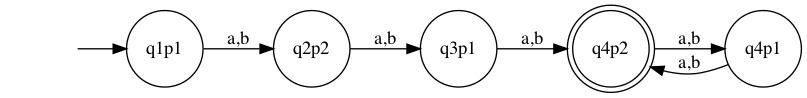
\includegraphics[width=0.8\textwidth]{g2_5_A1.png}
    \end{flushleft}
    \newpage
    Для удобства переименуем вершины обоих автоматов: \\ \\
    $L_2:$
    \begin{flushleft}
        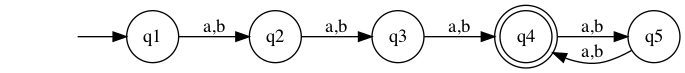
\includegraphics[width=0.8\textwidth]{g2_5_A.png}
    \end{flushleft}
    $\overline L_3:$
    \begin{flushleft}
        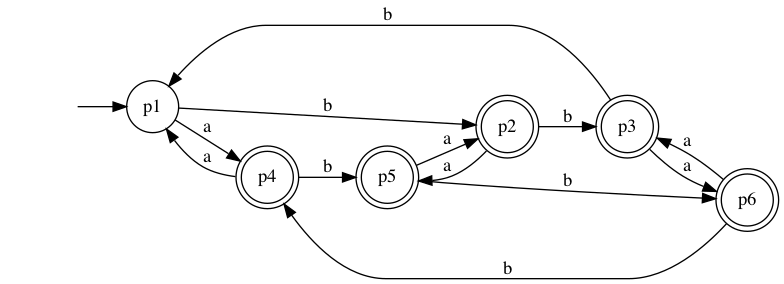
\includegraphics[width=0.8\textwidth]{g2_5_B.png}
    \end{flushleft}
    Разбираемся с произведением:
    $L_5 = L_2 \times \overline L_3$ \\
    $\sum = \{a, b\}$ \\
    $Q = \{q1p1, q1p2, q1p3, q1p4, q1p5, q1p6, q2p1, q2p2, q2p3, q2p4, q2p5, q2p6, q3p1, q3p2, q3p3, q3p4, q3p5, q3p6, q4p1, \\ q4p2, q4p3, q4p4, q4p5, q4p6, q5p1, q5p2, q5p3, q5p4, q5p5, q5p6,\}$ \\
    $s = \langle q1, p1 \rangle $ \\
    $T = \{q4p2, q4p3, q4p4, q4p5, q4p6\}$ \\ \\
    Для удобства сделаем три таблицы: \\ \\
    \begin{tabular}{|c|c|c|}
        \hline
                              & a                         & b     \\ \hline
         $\langle q1,p1 \rangle$    & $\langle q2,p4 \rangle$   & $\langle q2,p2 \rangle$    \\
         $\langle q1,p2 \rangle$    & $\langle q2,p5 \rangle$   & $\langle q2,p3 \rangle$    \\ 
         $\langle q1,p3 \rangle$    & $\langle q2,p6 \rangle$   & $\langle q2,p1 \rangle$    \\
         $\langle q1,p4 \rangle$    & $\langle q2,p1 \rangle$   & $\langle q2,p5 \rangle$    \\ 
         $\langle q1,p5 \rangle$    & $\langle q2,p2 \rangle$   & $\langle q2,p6 \rangle$    \\
         $\langle q1,p6 \rangle$    & $\langle q2,p3 \rangle$   & $\langle q2,p5 \rangle$    \\  \hline
         %%%%%%%%%%%%%%%%%%%%%%%%%%%%%%%%%%%%%%%%%%%%%%%%%%%%%%%%%%%%%%%%%%%%%%%%
         $\langle q2,p1 \rangle$    & $\langle q3,p4 \rangle$   & $\langle q3,p2 \rangle$    \\
         $\langle q2,p2 \rangle$    & $\langle q3,p5 \rangle$   & $\langle q3,p3 \rangle$    \\ 
         $\langle q2,p3 \rangle$    & $\langle q3,p6 \rangle$   & $\langle q3,p1 \rangle$    \\
         $\langle q2,p4 \rangle$    & $\langle q3,p1 \rangle$   & $\langle q3,p5 \rangle$    \\ 
         $\langle q2,p5 \rangle$    & $\langle q3,p2 \rangle$   & $\langle q3,p6 \rangle$    \\
         $\langle q2,p6 \rangle$    & $\langle q3,p3 \rangle$   & $\langle q3,p5 \rangle$    \\  \hline
    \end{tabular} \
    \begin{tabular}{|c|c|c|}
        \hline
                              & a                         & b     \\ \hline
         $\langle q3,p1 \rangle$    & $\langle q4,p4 \rangle$   & $\langle q4,p2 \rangle$    \\
         $\langle q3,p2 \rangle$    & $\langle q4,p5 \rangle$   & $\langle q4,p3 \rangle$    \\ 
         $\langle q3,p3 \rangle$    & $\langle q4,p6 \rangle$   & $\langle q4,p1 \rangle$    \\
         $\langle q3,p4 \rangle$    & $\langle q4,p1 \rangle$   & $\langle q4,p5 \rangle$    \\ 
         $\langle q3,p5 \rangle$    & $\langle q4,p2 \rangle$   & $\langle q4,p6 \rangle$    \\
         $\langle q3,p6 \rangle$    & $\langle q4,p3 \rangle$   & $\langle q4,p5 \rangle$    \\  \hline
         %%%%%%%%%%%%%%%%%%%%%%%%%%%%%%%%%%%%%%%%%%%%%%%%%%%%%%%%%%%%%%%%%%%%%%%%
         $\langle q4,p1 \rangle$    & $\langle q5,p4 \rangle$   & $\langle q5,p2 \rangle$    \\
         $\langle q4,p2 \rangle$    & $\langle q5,p5 \rangle$   & $\langle q5,p3 \rangle$    \\ 
         $\langle q4,p3 \rangle$    & $\langle q5,p6 \rangle$   & $\langle q5,p1 \rangle$    \\
         $\langle q4,p4 \rangle$    & $\langle q5,p1 \rangle$   & $\langle q5,p5 \rangle$    \\ 
         $\langle q4,p5 \rangle$    & $\langle q5,p2 \rangle$   & $\langle q5,p6 \rangle$    \\
         $\langle q4,p6 \rangle$    & $\langle q5,p3 \rangle$   & $\langle q5,p5 \rangle$    \\  \hline
    \end{tabular} \
    \begin{tabular}{|c|c|c|}
        \hline
                              & a                         & b     \\ \hline
         $\langle q5,p1 \rangle$    & $\langle q4,p4 \rangle$   & $\langle q4,p2 \rangle$    \\
         $\langle q5,p2 \rangle$    & $\langle q4,p5 \rangle$   & $\langle q4,p3 \rangle$    \\ 
         $\langle q5,p3 \rangle$    & $\langle q4,p6 \rangle$   & $\langle q4,p1 \rangle$    \\
         $\langle q5,p4 \rangle$    & $\langle q4,p1 \rangle$   & $\langle q4,p5 \rangle$    \\ 
         $\langle q5,p5 \rangle$    & $\langle q4,p2 \rangle$   & $\langle q4,p6 \rangle$    \\
         $\langle q5,p6 \rangle$    & $\langle q4,p3 \rangle$   & $\langle q4,p5 \rangle$    \\  \hline
         %%%%%%%%%%%%%%%%%%%%%%%%%%%%%%%%%%%%%%%%%%%%%%%%%%%%%%%%%%%%%%%%%%%%%%%%
    \end{tabular}
    \begin{flushleft}
        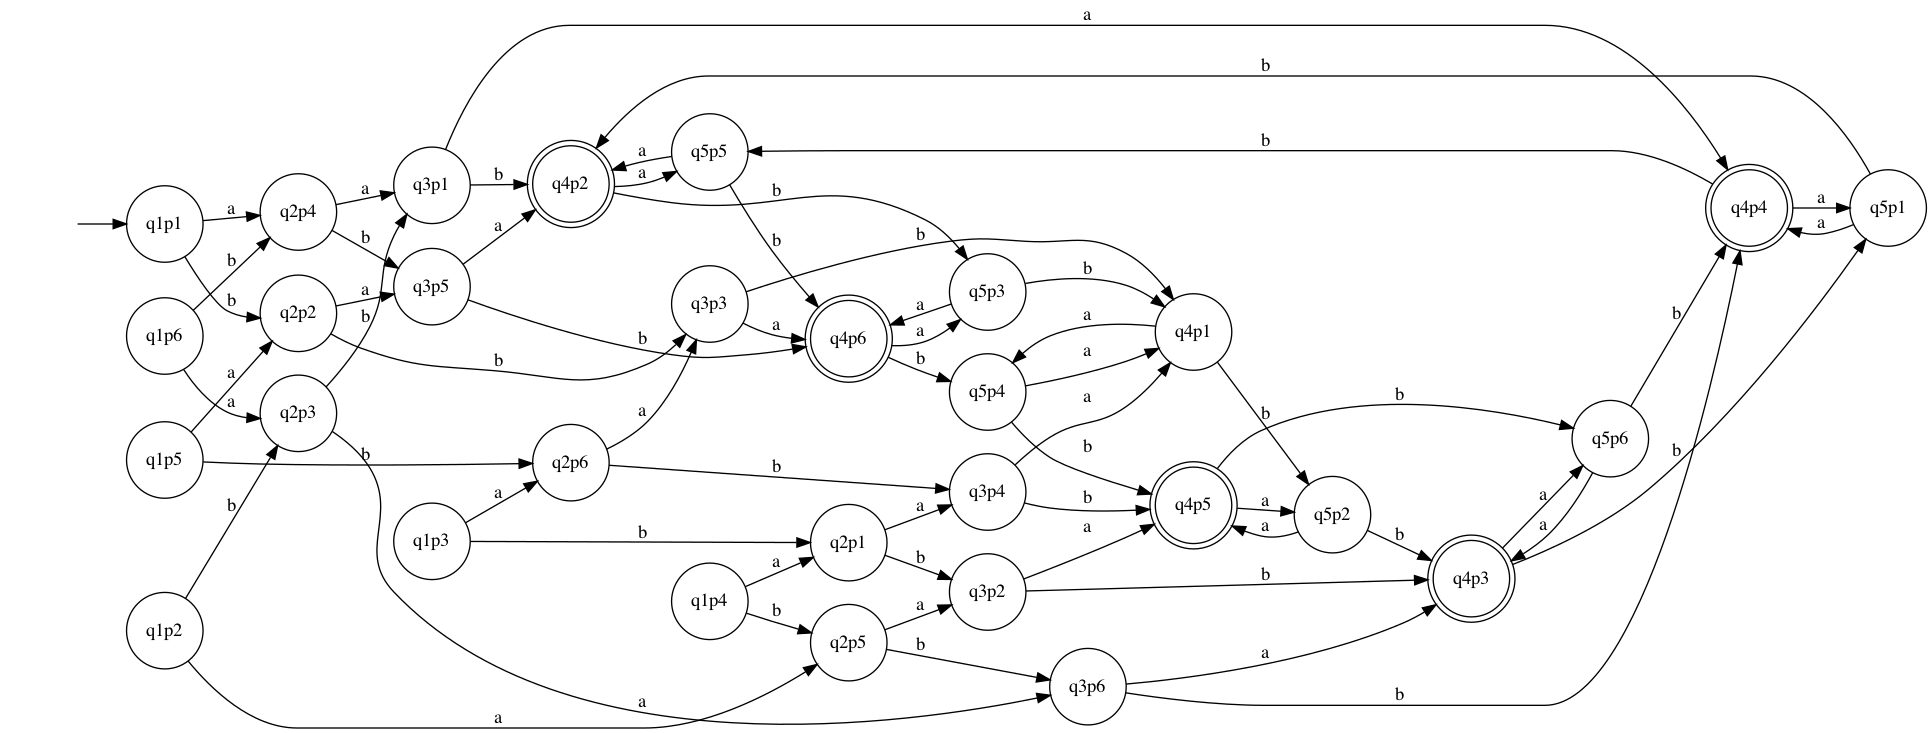
\includegraphics[width=0.9\textwidth]{g2_5.png}
    \end{flushleft}
\end{enumerate}

\section{Задание №3. Построить минимальный ДКА по регулярному выражению.}
\begin{enumerate}
    %% 3.1
    \item {$(ab + aba)^*a$} \\ \\ 
    \text{Построим НКА:}
    \begin{flushleft}
        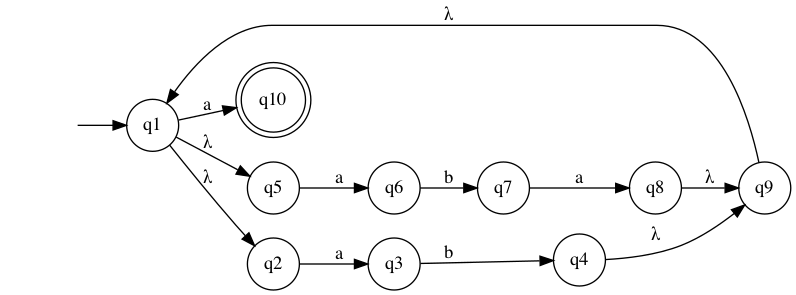
\includegraphics[width=0.85\textwidth]{g3_1_nka.png}
    \end{flushleft}
    \text{Избавимся от $\lambda$-переходов и примененим алгоритм Томпсона:} \\ \\
    \begin{flushleft}
        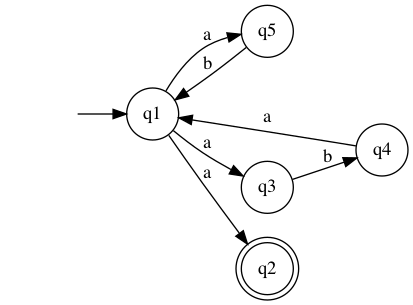
\includegraphics[width=0.45\textwidth]{g3_1_nka2.png}
    \end{flushleft}
    \begin{tabular}{|c|c|c|}
        \hline
         Q              & a             & b     \\ \hline
         q1             & q2 q3 q5      & -     \\
         q2 q3 q5       & -             & q1 q4 \\
         q1 q4          & q1 q2 q3 q5   & -     \\ 
         q1 q2 q3 q5    & q2 q3 q5      & q1 q4 \\ \hline
    \end{tabular} \\ \\
    По данной таблице видно, что при построении ДКА он будет минимальным. 
    \text{Построим ДКА:}\\ 
    \begin{flushleft}
        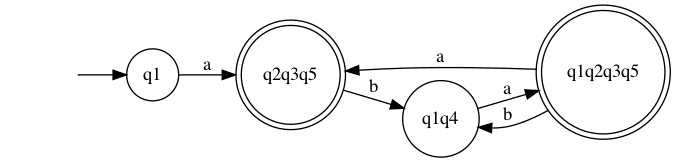
\includegraphics[width=0.9\textwidth]{g3_1.png}
    \end{flushleft}
    %% 3.2
    \item {$a(a(ab)^*b)^*(ab)^*$} \\ \\
    \text{Построим НКА:}
    \begin{flushleft}
        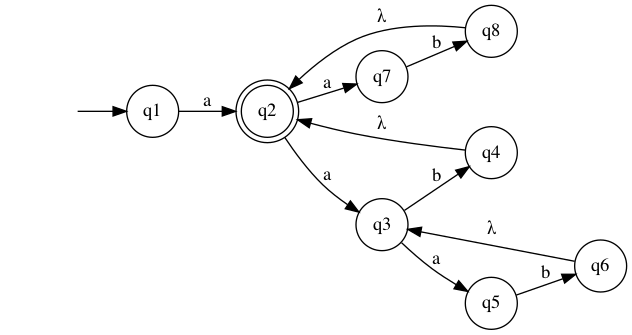
\includegraphics[width=0.9\textwidth]{g3_2_nka.png}
    \end{flushleft}
    \text{Избавимся от $\lambda$-переходов и примененим алгоритм Томпсона:} \\ \\
    \begin{flushleft}
        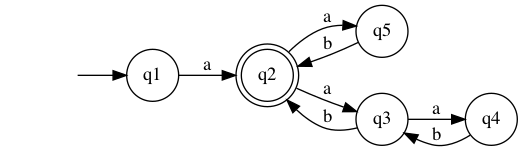
\includegraphics[width=0.9\textwidth]{g3_2_nka2.png}
    \end{flushleft}
    \begin{tabular}{|c|c|c|}
        \hline
         Q          & a             & b     \\ \hline
         q1         & q2            & -     \\
         q2         & q3 q5         & -     \\
         q3 q5      & q4            & q2    \\ 
         q4         & -             & q3    \\
         q3         & q4            & q2    \\ \hline
    \end{tabular} \\
    
    \text{Построим ДКА:}\\ 
    \begin{flushleft}
        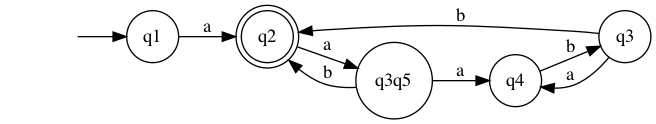
\includegraphics[width=0.9\textwidth]{g3_2.png}
    \end{flushleft}
    Однако это не минимальный ДКА. По таблице в алгоритме Томпсона $3 \text{и} 5$ строки совпадают, следовательно вершины можно объединить с сохранением переходов. Получим минимальный ДКА:
    \begin{flushleft}
        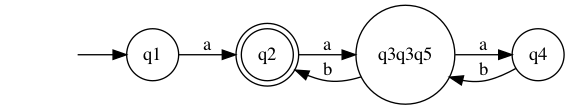
\includegraphics[width=0.9\textwidth]{g3_2_fin.png}
    \end{flushleft}
    %% 3.3
    \item {$(a + (a + b)(a + b)b)^*$} \\ \\
    \text{Построим НКА:}
    \begin{flushleft}
        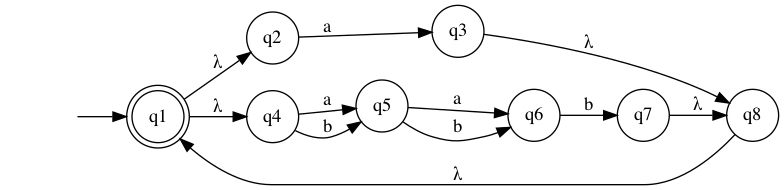
\includegraphics[width=0.9\textwidth]{g3_3_nka.png}
    \end{flushleft}
    \text{Избавимся от $\lambda$-переходов и примененим алгоритм Томпсона:} \\ \\
    \begin{flushleft}
        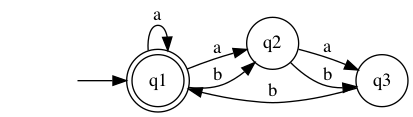
\includegraphics[width=0.8\textwidth]{g3_3_nka2.png}
    \end{flushleft}
    \begin{tabular}{|c|c|c|}
        \hline
         Q              & a             & b         \\ \hline
         q1             & q1 q2         & q2        \\
         q1 q2          & q1 q2 q3      & q2 q3     \\
         q2             & q3            & q3        \\ 
         q1 q2 q3       & q1 q2 q3      & q1 q2 q3  \\
         q3             & -             & q1        \\ 
         q2 q3          & q3            & q1 q3     \\ 
         q1 q3          & q1 q2         & q2 q3     \\ \hline
    \end{tabular} \\ \\
    По данной таблице видно, что при построении ДКА он будет минимальным.
    \text{Построим ДКА:}\\ 
    \begin{flushleft}
        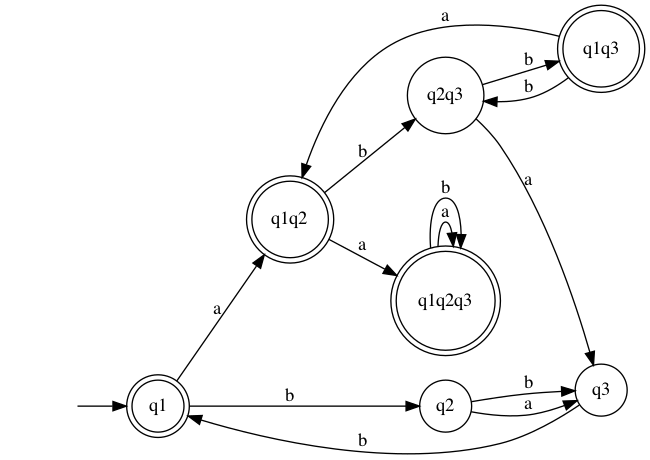
\includegraphics[width=0.9\textwidth]{g3_3.png}
    \end{flushleft}
    \newpage
    %% 3.4
    \item {$(b + c)((ab)^*c + (ba)^*)^*$} \\ \\
    \text{Построим НКА:}
    \begin{flushleft}
        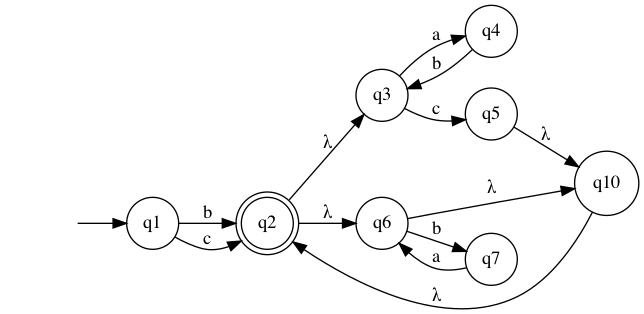
\includegraphics[width=0.9\textwidth]{g3_4_nka.png}
    \end{flushleft}
    Избавимся от $\lambda$-переходов и примененим алгоритм Томпсона. \\ \\
    \textit{Замечание.} В процессе избавления от $\lambda$-переходов получил ДКА:
    \begin{flushleft}
        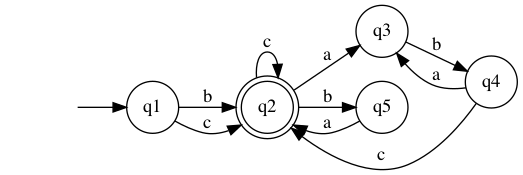
\includegraphics[width=0.8\textwidth]{g3_4.png}
    \end{flushleft}
    Убедимся в том, что он минимальный: \\ \\
    \begin{tabular}{|c|c|c|c|}
        \hline
         Q              & a             & b         & c     \\ \hline
         q1             & -             & q2        & q2    \\
         q2             & q3            & q5        & q2    \\
         q3             & -             & q4        & -     \\ 
         q4             & q3            & -         & q2    \\
         q5             & q2            & -         & -     \\ 
         \hline
    \end{tabular} \\ \\
    %% 3.5
    \item {$(a + b)^+ (aa + bb + abab + baba)(a + b)^+$} \\ \\
    \text{Построим НКА:}
    \begin{flushleft}
        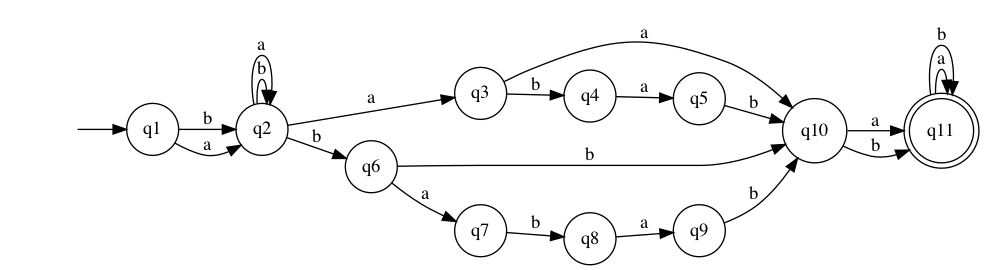
\includegraphics[width=0.9\textwidth]{g3_5_nka.png}
    \end{flushleft}
    \text{Примененим алгоритм Томпсона:} \\ \\
    \begin{tabular}{|c|c|c|c|}
         \hline
         Q              & a             & b             \\ \hline
         q1             & q2            & q2            \\
         q2             & q2 q3         & q2 q6         \\
         q2 q3          & q2 q3 q10     & q2 q6 q4      \\ 
         \hline
    \end{tabular} \\ \\
    На этом моменте я понял, что эта таблица будет нереально огромной и из-за этого повыситься вероятность допущения ошибки. Поэтому начал строить у себя постепенно сразу ДКА и исправлять.
    \text{Построим ДКА:}\\ 
    \begin{flushleft}
        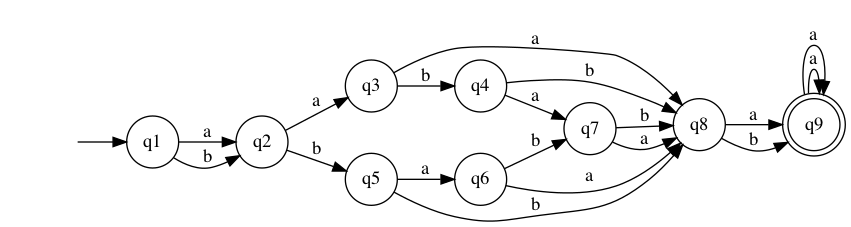
\includegraphics[width=0.9\textwidth]{g3_5.png}
    \end{flushleft}
\end{enumerate}c

\section{Задание №4. Определить является ли язык регулярным или нет.}
\begin{enumerate}
    %% 4.1 
    \item {$L = \{ (aab)^n b(aba)^m \ | \ n \geq 0, m \geq 0 \}$} \\ \\
    Данный язык является регулярным. Построим ДКА:
    \begin{flushleft}
        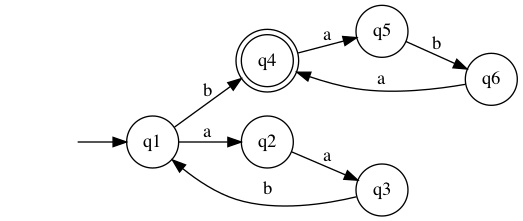
\includegraphics[width=0.8\textwidth]{g4_1.png}
    \end{flushleft}
    %% 4.2
    \item {$L = \{ uaav \ | \ u \in \{ a,b\}^*, v \in \{a, b\}^*, |u|_b \geq |u|_a \}$} \\ \\
    Зафиксируем $\forall n > 0$. Возьмем слово $w = b^n aa a^n$. Будем проверять его по лемме:
    $$ |w| = n + 2 + n \geq n, \quad w = xyz $$ 
    Пусть $p \leq n$ и $p > 0 $. Тогда составим разбиение:
    $$ x = b^{n-p} $$
    $$ y = b^p $$
    $$ z = aaa^n $$
    $$ |xy| = p + n - p \leq n $$
    $$ |y| = p \geq 1 $$
    По лемме: $\forall k \geq 0$,  $xy^kz \in L$.
    Возьмем $ k = 0 $. Тогда:
    $$ xy^0z = b^{n-p}b^0aaa^n = b^{n-p}aaa^n $$
    В силу того, что $ p > 0 $, следует, что $ |u|_b < |u|_a $, что противоречит языку. Лемма не выполнилась при $k = 0$, а значит $L$ - не регулярный язык.
    %% 4.3
    \item {$L = \{ a^mw \ | \ w \in \{ a,b \}^*, 1 \leq |w|_b \leq m \}$} \\ \\
    Зафиксируем $\forall n > 0$. Возьмем слово $w = a^n b^n$. Будем проверять его по лемме:
    $$ |w| = n + n \geq n, \quad w = xyz $$ 
    Пусть $p < n$ и $ p > 0 $. Тогда составим разбиение:
    $$ x = a^{n-p} $$
    $$ y = a^p $$
    $$ z = b^n $$
    $$ |xy| = p + n - p \leq n $$
    $$ |y| = p \geq 1 $$
    По лемме: $\forall k \geq 0$,  $xy^kz \in L$.
    Возьмем $ k = 0 $. Тогда:
    $$ xy^0z = a^{n-p}a^0b^n = a^{n-p}b^n $$
    В силу того, что $ p > 0 $, следует, что $ n-p < n $. Это означает, что лемма не выполнилась при $ k = 0 $ (по условию $1 \leq |w|_b \leq m$, а вышло $m = n-p$ и $|w|_b = n$), а значит $L$ - не регулярный язык.
    %% 4.4
    \item {$L = \{ a^k b^m a^n \ | \ k = n \vee m > 0 \}$} \\ \\
    Зафиксируем $\forall n > 0$. Возьмем слово $w = a^n b a^n$. Будем проверять его по лемме:
    $$ |w| = n + 1 + n \geq n, \quad w = xyz $$ 
    Пусть $ p \leq n$ и $ p > 0 $. Тогда составим разбиение:
    $$ x = a^{n - p} $$
    $$ y = a^p $$
    $$ z = b a^n $$
    $$ |xy| = n - p + p \leq n $$
    $$ |y| = p \geq 1 $$
    По лемме: $\forall j \geq 0$,  $xy^jz \in L$.
    Будем накачивать по $j$:
    $$ xy^jz = a^{n - p} a^{pj} b a^n = a^{n - p + pj}b a^n = a^{n + p(j-1)}b a^n$$
    Обратимся к языку. Изначальное условие $ k = n \vee m > 0 $. На нашей получившейся накачке $ m = 1 $, $ n $ остается $ n > 0 $. Тогда $ k = n \vee 1 > 0 $. А мы получили, что $ k = n + p(j-1)$. При $j > 1$ получаем противоречие, а значит лемма не выполняется $ \xrightarrow[]{}$ язык не регулярный. 
    %% 4.5
    \item {$L = \{ ucv \ | \ u \in \{ a,b \}^*, v \in \{ a,b\}^* , u \neq v^R \}$ } \\ \\
    Докажем не регулярность языка через $\overline L$. \\ \\
    $\overline L = \{ ucv \ | \ u \in \{ a,b \}^*, v \in \{ a,b\}^* , u = v^R \}$ \\ \\
    Зафиксируем $\forall n > 0$. Возьмем слово $w = a^{n} c a^{n}$. Будем проверять его по лемме:
    $$ |w| = n + 1 + n \geq n, \quad w = xyz $$ 
    Пусть $ p \leq n$ и $ p > 0 $. Тогда составим разбиение:
    $$ x = a^{n - p} $$
    $$ y = a^p $$
    $$ z = c a^n $$
    $$ |xy| = n - p + p \leq n $$
    $$ |y| = p \geq 1 $$
    По лемме: $\forall k \geq 0$,  $xy^kz \in L$.
    Будем накачивать по $k$:
    $$ xy^kz = a^{n - p} a^{pk} c a^n = a^{n - p + pk} c a^n = a^{n + p(k-1)} c a^n $$
    Обратимся к языку. Изначальное условие обратного языка $ u = v^R $. На нашей получившейся накачке $ u = a^{n+p(k-1)} $, $ v^R = a^n $. Тогда при $k > 1$ условие $ u = v^R $ не выполняется. Получено противоречие, а значит лемма не выполняется $ \xrightarrow[]{}$ язык $\overline L$ не регулярный $ \xrightarrow[]{}$ язык $L$ не регулярный.
\end{enumerate}
\end{document}